\documentclass[11pt]{article}

% ---------- Packages ----------
\usepackage[a4paper,margin=1in]{geometry}
\usepackage{graphicx}
\usepackage{microtype}
\usepackage{amsmath,amssymb}
\usepackage{placeins}
\usepackage{booktabs}
\usepackage{fontawesome5}
\usepackage{hyperref}
\usepackage{caption}
\usepackage{subcaption}
\usepackage[superscript]{cite}
\usepackage{array}

\usepackage{setspace}
\onehalfspacing

% TikZ for the pipeline figure
\usepackage{tikz}
\usetikzlibrary{arrows.meta,positioning}

% ---------- Metadata ----------
\title{Alignment-Free Detection of Horizontal Gene Transfer Candidates\\
via Protein Similarity Graphs and Anomaly Scoring}

\author{}
\date{}

\begin{document}
\maketitle
\vspace{-52pt}

\begin{center}
\renewcommand{\arraystretch}{1.15}
\setlength{\tabcolsep}{10pt}

\begin{tabular}{c@{\hspace{2.8cm}}c}
{\normalsize\textbf{Roee Tekoah}} &
{\normalsize\textbf{Noam Korkos}} \\[2pt]
\footnotesize\texttt{roee.tekoah@mail.huji.ac.il} &
\footnotesize\texttt{noam.korkos@mail.huji.ac.il}
\end{tabular}

\vspace{16pt}

{\small\itshape
The Rachel and Selim Benin School of Computer Science and Engineering\\
The Hebrew University of Jerusalem
}\\[8pt]
\faGithub\ \href{https://github.com/MY-REPO/}{\texttt{Project repository}}\\[10pt]
{\small February 2026}
\end{center}

\begin{abstract}
Horizontal gene transfer (HGT) is a major driver of microbial evolution, yet detecting HGT at scale remains challenging due to the computational cost and complexity of alignment- and phylogeny-based methods. We present a scalable, alignment-free pipeline for identifying HGT candidates in large protein collections using sparse protein similarity graphs and graph-based anomaly analysis. Proteins are compared via \textit{k}-mer overlap, normalized using robust statistics to account for species-specific background similarity, and embedded in a graph structure that enables detection of structurally anomalous cross-species similarity patterns. Applying the method to RefSeq bacterial proteins reveals distinct connectivity regimes, including dense multi-taxa exchange modules, chained transfer-like structures, and localized high-confidence bridges. Our results demonstrate that graph-based structural context provides a powerful and interpretable signal for prioritizing HGT candidates suitable for downstream biological validation.
\end{abstract}

\setlength{\textfloatsep}{10pt}
\setlength{\floatsep}{8pt}
\setlength{\intextsep}{8pt}

% =========================
% 1. Introduction
% =========================
\section{Introduction}

Horizontal gene transfer (HGT) is a central driver of microbial evolution, enabling rapid
acquisition of adaptive functions such as antibiotic resistance and novel metabolic capabilities \cite{Koonin2001,Davies2000}. Detecting HGT at scale remains challenging because classical approaches based on sequence alignment and phylogenetic reconstruction require expensive inference procedures and are difficult to apply exhaustively to large protein collections \cite{Ragan2001,Philippe2011}. Large curated resources such as NCBI RefSeq therefore motivate scalable screening methods that prioritize suspicious cross-species similarities for downstream validation \cite{OLeary2016}.

Our central research question is whether species-pair–aware normalization combined with graph structural context can reliably prioritize horizontal gene transfer candidates at scale without reliance on alignment or phylogenetic reconstruction.

We present an alignment-free pipeline for large-scale HGT candidate discovery based on sparse
protein similarity graphs. Protein pairs are proposed via \textit{k}-mer overlap, cross-species similarity is normalized relative to species-pair baselines using robust statistics, and graph-based anomaly analysis prioritizes proteins whose similarities are both unusually strong and embedded in structurally informative cross-taxon contexts.

Our contributions are threefold. First, we introduce a species-pair–aware normalization scheme
based on robust statistics that calibrates cross-species similarity relative to heterogeneous
background conservation levels. Second, we combine local anomaly evidence with graph-structural
features in a gated, component-aware ranking framework that suppresses generic conserved
proteins while prioritizing structurally informative candidates. Third, we demonstrate that sparse similarity graphs reveal distinct and interpretable connectivity regimes consistent with different transfer-like patterns at scale.

Unlike global-threshold similarity approaches, our framework explicitly calibrates similarity
relative to species-pair baselines and integrates structural graph context into candidate ranking.


% =========================
% 2. Data
% =========================
\section{Data}

\subsection{Data source and species selection}
We constructed our dataset from the NCBI RefSeq protein database, focusing on a curated set of bacterial species. Assembly metadata were obtained from the RefSeq assembly summary and filtered to retain high-quality genomes (Complete Genome or Chromosome level), prioritizing reference and representative assemblies.

To control dataset size, we selected up to two assemblies per species using a deterministic ranking. While this choice ensured manageable scale and consistent annotation quality, it introduced some redundancy due to near-identical assemblies; we discuss this limitation in Section~\ref{sec:discussion}.

\subsection{Protein extraction and preprocessing}
Protein FASTA files were downloaded from RefSeq and parsed into a unified table containing protein identifiers, species labels, and sequence lengths. Proteins shorter than 50 amino acids were excluded to reduce spurious similarity arising from short or low-complexity sequences. The final dataset contains approximately 324{,}000 proteins across 50 species. The selected 50 species provide a manageable yet taxonomically diverse testbed; scaling to larger collections is enabled by the sparsity and modular design of the pipeline.

% =========================
% 3. Method
% =========================
\section{Method}

An overview of the pipeline is shown in Figure~\ref{fig:pipeline_overview}.

\begin{figure}[p]
\centering
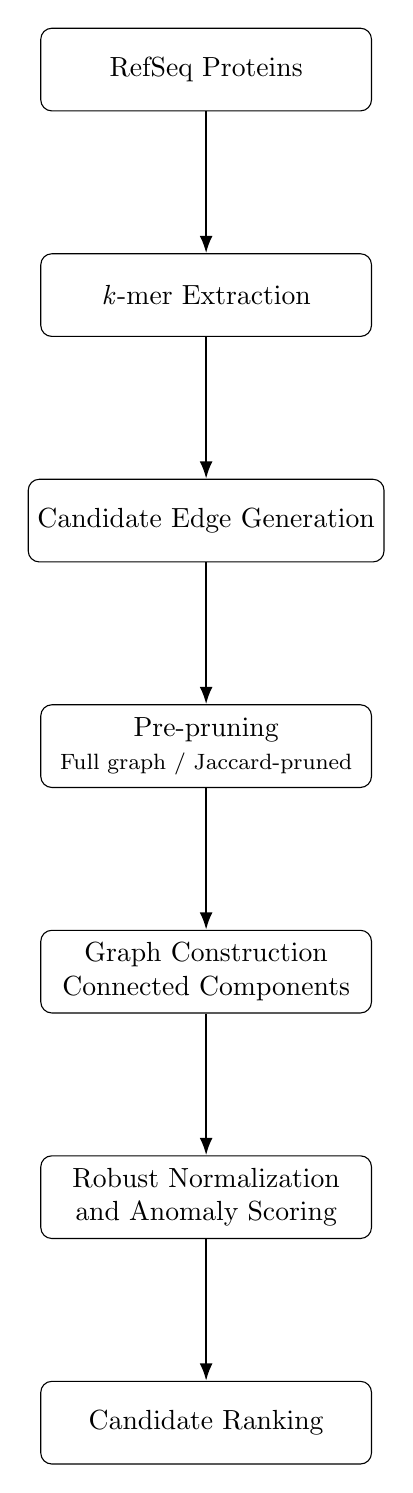
\begin{tikzpicture}[
    node distance=1.8cm,
    box/.style={draw, rectangle, rounded corners, align=center,
                minimum width=4.2cm, minimum height=1.05cm},
    arrow/.style={-{Latex[length=2.2mm]}, thick}
]
\node[box] (data) {RefSeq Proteins};
\node[box, below=of data] (kmers) {\textit{k}-mer Extraction};
\node[box, below=of kmers] (cand) {Candidate Edge Generation};
\node[box, below=of cand] (prune) {Pre-pruning\\{\footnotesize Full graph / Jaccard-pruned}};
\node[box, below=of prune] (graph) {Graph Construction\\Connected Components};
\node[box, below=of graph] (score) {Robust Normalization\\and Anomaly Scoring};
\node[box, below=of score] (rank) {Candidate Ranking};

\draw[arrow] (data) -- (kmers);
\draw[arrow] (kmers) -- (cand);
\draw[arrow] (cand) -- (prune);
\draw[arrow] (prune) -- (graph);
\draw[arrow] (graph) -- (score);
\draw[arrow] (score) -- (rank);
\end{tikzpicture}
\caption{Overview of the HGT candidate detection pipeline. Protein sequences are represented using \textit{k}-mers to
generate cross-species similarity candidates. Pre-pruning controls graph density by retaining high-confidence
edges, after which robust normalization and graph-based anomaly scoring are applied to identify candidate
HGT-related proteins.}
\label{fig:pipeline_overview}
\end{figure}

\subsection{Similarity Candidate Generation}
To avoid computationally infeasible all-vs-all alignments, proteins shorter than 50 amino acids were excluded and remaining sequences were represented as sets of distinct \textit{k}-mers ($k=6$), encoded as collision-free base-20 integers over the canonical amino acid alphabet\cite{Sims2009,Haubold2014}.

To suppress non-informative overlaps, highly frequent \textit{k}-mers (posting list size $>100$) were excluded. Candidate pairs required $\ge6$ shared k-mers. Only cross-species pairs were considered, as intra-species similarity is expected and not informative for HGT detection, and candidate lists were capped to the top 10 matches per protein. Exact Jaccard similarity over the \textit{k}-mer sets was then computed for these candidate pairs to obtain deterministic similarity scores. Sketching approaches such as MinHash could further scale the pipeline to larger datasets\cite{Broder1997,Ondov2016}.

\subsection{Graph Construction and Pruning}
Candidate pairs were assembled into an undirected, weighted similarity graph, with edges weighted by Jaccard similarity of \textit{k}-mer sets. Similarities were normalized per species pair by retaining the strongest edges (top 10\% per pair). All retained edges were required to meet an absolute minimum Jaccard similarity of 0.1, and per-node degree was capped at 20.


Additional taxonomic distance filters retained edges with taxonomic distance in the range [2,4]. These steps reduced the graph from approximately $9\times 10^5$ candidate edges to 92{,}790 edges, yielding the sparse graph analyzed below.

\subsection{Graph-Based Anomaly Scoring}
Graph structure enables evaluation of anomalous similarity within mixed-species components. Similarity scores were normalized using robust z-scores based on the median and MAD\cite{Rousseeuw1993}, computed per species pair when $\ge30$ edges were available.

Connected components of the pruned graph were analyzed. 
Taxonomic mixing was quantified using species count and normalized Shannon entropy. Anomaly concentration was measured as the fraction of edges with $z\ge3$. Node features included anomaly evidence (max and top-k mean z-scores) and structural connectivity metrics: cross-species degree, neighbor entropy, participation coefficient\cite{Guimera2005}, clustering coefficient, and betweenness centrality.

Proteins were ranked using a component-aware scoring framework with threshold gates requiring sufficient component size, taxonomic mixing, anomalous similarity, and cross-species connectivity (component size $\ge10$, entropy $\ge0.75$, node degree $\ge4$, mean top-5 $z\ge2$).

\begin{equation}
\log S(u) = \log \Phi(C_u) + \log A(u) + \log T(u),
\end{equation}

$\Phi(C_u)$ captures component-level taxonomic mixing and anomaly concentration, $A(u)$ aggregates normalized similarity scores, and $T(u)$ summarizes cross-species connectivity and bridge-like topology. To stabilize scale differences across components, aggregation was performed in log-space, so high scores arise only when anomaly and structural evidence co-occur.

% =========================
% 4. Results
% =========================
\section{Results}

\subsection{Graph scale and impact of pre-pruning}

\begin{figure}[!t]
    \centering
    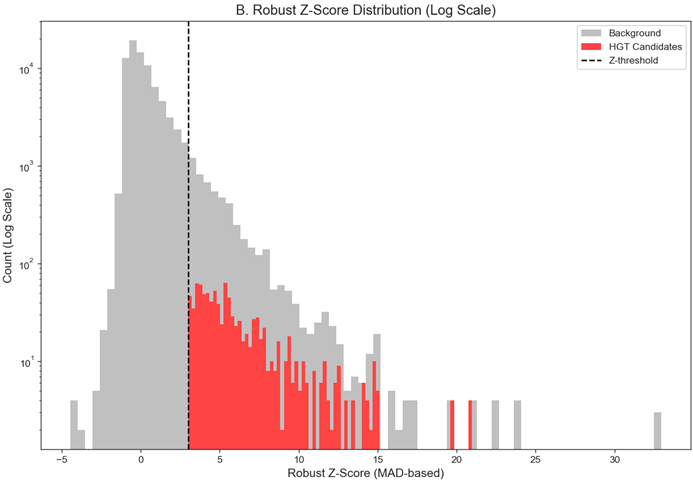
\includegraphics[width=0.5\linewidth]{figures/z_score_distribution.png}
    \caption{Distribution of MAD-based Z-score for all protein-protein edges, plotted in logarithmic y-axis. The background distribution (grey) represents the global set of 911,306 edges, which clusters near the median (Z~0), reflecting expected evolutionary divergence. The dashed black line is the statistical significance threshold (Z=3). Edges connected to the final HGT candidates (red) are localized to the right tail of the distribution.}
    \label{fig:zscoredist}
\end{figure}

The full candidate graph contains 911{,}306 cross-species edges over 214{,}136 proteins. After Jaccard-based pre-pruning it contains 92{,}790 edges over 37{,}421 proteins across 5,262 connected components.

Component size is highly skewed (median 4; 95th percentile 20; max 107). Median components span two species, and only 18.5\% contain $\ge5$ species.

Anomalous similarity is globally sparse: the median fraction of high-z edges per component is 0 and only 3.9\% of components show substantial anomaly concentration ($high\_z\_frac >0.3$). This sparsity is also evident in the global edge distribution (Figure~\ref{fig:zscoredist}), where most similarities cluster near the baseline while high-$z$ edges occupy a small right tail.

Across 37{,}421 proteins in the pruned graph, only 5.9\% satisfy the gating criteria and receive a non-zero score, indicating strong selectivity.

\subsection{Structural regimes in the Jaccard-pruned graph}

\begin{table}[t]
\centering
\small
\begin{tabular}{lrrrrrr}
\toprule
Component & Proteins & Edges & Density & Species & $H_{\mathrm{norm}}$ & high-$z$ frac \\
\midrule
5  & 97 & 632 & 0.136 & 50 & 0.998 & 0.60 \\
8  & 95 & 589 & 0.130 & 49 & 0.998 & 0.47 \\
32 & 71 & 332 & 0.134 & 31 & 0.958 & 0.063 \\
\bottomrule
\end{tabular}
\caption{Summary statistics for representative components in the pruned similarity graph.}
\label{tab:components}
\end{table}

\begin{figure}[!t]
  \centering
  \includegraphics[height=0.45\textheight]{figures/component_5.png}
  \caption{Component 5: Broad multi-taxa exchange module. Nodes represent proteins and edges represent cross-species similarity. Node size reflects candidate score, and highlighted edges correspond to high-surprise similarities relative to species-pair baselines.}
  \label{fig:component5}
\end{figure}

\begin{figure}[!t]
  \centering
  \includegraphics[height=0.45\textheight]{figures/component_8.png}
  \caption{Component 8: Chained cross-species connectivity. Compact sub-clusters are linked by a small number of high-surprise edges, producing elongated paths across distant taxa.}
  \label{fig:component8}
\end{figure}

\begin{figure}[t]
  \centering
  \includegraphics[width=\linewidth]{figures/component_32.png}
  \caption{Component 32: Localized high-confidence bridges. Two coherent regions are connected by a small number of strong cross-species edges, with anomalous signal concentrated in the bridges.}
  \label{fig:component32}
\end{figure}

Three representative components illustrate distinct structural regimes of cross-species similarity (Table~\ref{tab:components}).
Component 5 forms a dense multi-taxa exchange module spanning many species with near-maximal entropy and strong anomaly concentration (Table~\ref{tab:components}, Figure~\ref{fig:component5}). High-scoring proteins participate in multiple cross-species interactions, suggesting a shared exchange module rather than isolated anomalies.

Clusters within this component correspond to horizontally transferred ribosomal proteins. 
The left cluster involves ribosomal protein S21, which has been linked to late-stage phage replication and can become part of the phage genetic toolkit used to hijack host translational machinery after transfer \cite{phage_S21_hgt,frontiers_hgt_tools}. 
In contrast, the top and right clusters correspond to ribosomal protein S12 (encoded by \textit{rpsL}) within the 30S ribosomal subunit, whose mutations are associated with streptomycin resistance \cite{rpsL_streptomycin}.

Component 8 shows a chained transfer-like topology spanning many taxa with high entropy and substantial anomaly concentration (Table~\ref{tab:components}, Figure~\ref{fig:component8}). Compact subclusters are linked by a few high-surprise edges, producing elongated paths consistent with stepwise propagation across lineages. 

Clusters in this component correspond to horizontal transfer of the 30S ribosomal protein S10 (encoded by \textit{rpsJ}), whose mutations are known markers of tigecycline resistance\cite{rpsJ_tigecycline}. Horizontal transfer of this gene has been reported among \textit{Mycobacterium} species, including \textit{M. tuberculosis} \cite{mycobacterium_rpsJ_transfer}.

Component 32 instead exhibits localized high-confidence bridges across many species but with relatively low anomaly concentration (Table~\ref{tab:components}, Figure~\ref{fig:component32}). Here anomalous signal concentrates in a few bridging edges linking otherwise ordinary similarity neighborhoods. 

Clusters in this component correspond to horizontal transfer of glucose-1-phosphate thymidylyltransferase, a key enzyme in bacterial surface polysaccharide biosynthesis. Such polysaccharides contribute to host immune evasion; for example, Capnocytophaga (pathogenic oral commensal in dogs) species use them to resist the bactericidal effects of human serum\cite{capnocytophaga_surface_polysaccharide,capnocytophaga_serum_resistance}.

\subsection{Comparison with the full candidate graph}

Applying the same normalization and structural scoring to the full candidate graph yields substantially denser connectivity, with many additional proteins and edges that obscure component boundaries. This contrast supports pre-pruning as a practical requirement for interpreting anomalous similarity patterns at scale.

\subsection{Score distribution and selectivity}

Among the top 200 ranked proteins, the median score was 5.9 (IQR: 4.47–8.17), with the 95th percentile at 12.74 and a maximum of 18.76. These values represent the extreme upper tail of the scoring distribution among the 5.9\% of proteins that passed gating.

\FloatBarrier

% =========================
% 5. Discussion
% =========================
\section{Discussion}
\label{sec:discussion}

Our method is intended as a scalable hypothesis-generation framework rather than a definitive test for horizontal gene transfer. By replacing alignment and phylogenetic reconstruction with species-aware normalization and graph-structural analysis, we trade resolution for scalability, prioritizing candidates for downstream validation rather than directly confirming transfer events.

Several design choices reflect explicit trade-offs. Restricting candidate generation (k=6, $\ge6$ shared k-mers, posting lists $\ge100$, top-10 matches per protein) suppresses conserved motifs and ubiquitous housekeeping genes. While this substantially reduces false positives arising from generic conservation, it may also exclude true transfer events involving highly conserved or short protein domains. Similarly, per-species-pair percentile pruning (top 10\%) and degree capping (top 20 edges per node) improve structural interpretability but introduce heuristic thresholds that may affect sensitivity.

The robust $z$-score normalization mitigates heterogeneity across species pairs, yet its effectiveness depends on sufficient edge counts per pair (minimum 30). Rare species pairs with few observations may therefore yield unstable baselines. In addition, anomaly thresholds
(e.g., $z \ge 3$) emphasize extreme deviations and may bias the ranking toward dramatic cross-species similarities while overlooking subtler but biologically meaningful transfers.

False positives may arise from convergent evolution, ancient homologs, or unmodeled taxonomic structure. Conversely, false negatives may arise when transfer events occur between closely related taxa that were filtered by taxonomic distance thresholds, or when
post-transfer divergence reduces $k$-mer overlap below detection limits.

Despite these limitations, the consistency of signal across edge-level anomaly, node-level connectivity, and component-level taxonomic mixing suggests that high-ranking candidates are not artifacts of a single heuristic. Instead, they represent multi-scale structural deviations from expected background similarity.

Future validation should integrate orthogonal genomic evidence, including synteny conservation,
plasmid or genomic island association, and phylogenetic incongruence analysis. Sensitivity
analysis over $k$, pruning percentiles, and anomaly thresholds would further clarify robustness
and support scaling to larger protein collections.

\subsection{Limitations and detectability of ameliorated HGT}
\begin{figure}
    \centering
    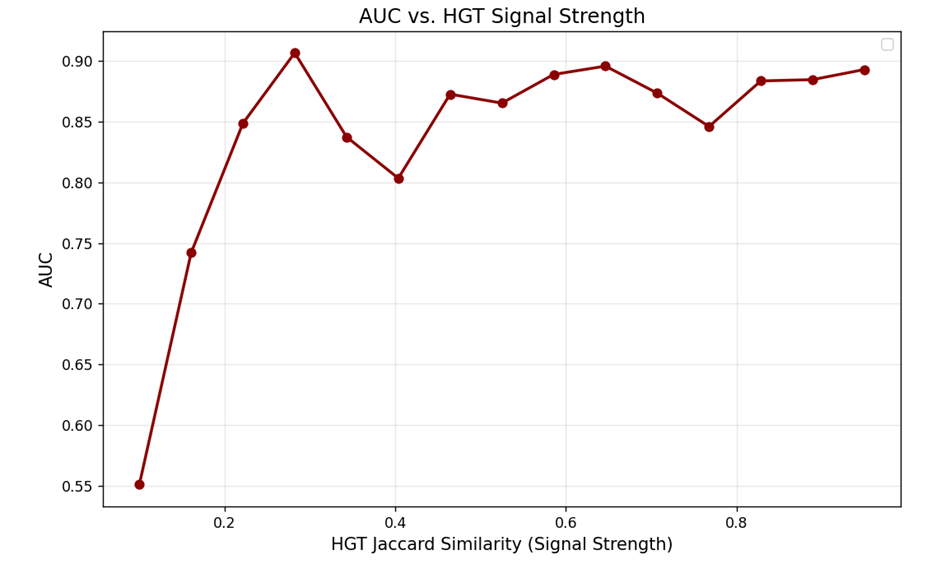
\includegraphics[width=0.8\linewidth]{figures/Genomic_Amelioration_Asses.png}
    \caption{AUC of the anomaly-detection pipeline as a function of injected HGT Jaccard similarity (used as a proxy for amelioration level). Simulations included 10 species (50 proteins each) with 30 injected HGT events. Detection remains strong for similarity $\ge0.20$ (AUC $>0.8$) but drops sharply below this threshold, indicating reduced sensitivity for highly ameliorated transfers.}
    \label{fig:amelioration_auc}
\end{figure}

To assess how genomic amelioration affects detectability, we simulated HGT events with varying Jaccard similarity while modeling conserved housekeeping genes with high similarity (0.75–0.95) and background proteins with low similarity. Because our filtering prioritizes high-similarity edges, strongly ameliorated transfers are increasingly discarded as background, suggesting that the method primarily detects relatively recent or moderately diverged HGT events.

As shown in Figure~\ref{fig:amelioration_auc}, performance declines rapidly as similarity decreases.

\subsection{Implementation and Reproducibility}

All scripts required to reproduce the analysis are available in github. The repository contains the exact configurations and intermediate artifacts used to produce
our results. The repository also contains online supplementary matriels. 

% =========================
% 6. Conclusion
% =========================
\section{Conclusion}

We presented a scalable, alignment-free framework for large-scale HGT candidate detection based on species-pair–aware normalization and sparse similarity graphs. By combining robust statistical calibration with graph-structural features and explicit gating criteria, the method selectively reduces large protein collections to a compact, interpretable set of high-priority candidates suitable for downstream phylogenetic and genomic validation.

% =========================
% References
% =========================
\bibliographystyle{unsrt}
\bibliography{references}

\end{document}
